\RequirePackage{luatex85}
\documentclass[tikz, border=10pt]{standalone}

\usepackage[compat=1.1.0]{tikz-feynman}

\newcommand{\Ptop}{\ensuremath{\mathrm{t}}}
\newcommand{\Pg}{\ensuremath{\mathrm{g}}}
\newcommand{\Pb}{\ensuremath{\mathrm{b}}}
\newcommand{\Pq}{\ensuremath{\mathrm{q}}}
\newcommand{\PH}{\ensuremath{\mathrm{H}}}
\newcommand{\PW}{\ensuremath{\mathrm{W}}}
\newcommand{\PZ}{\ensuremath{\mathrm{Z}}}

\begin{document}

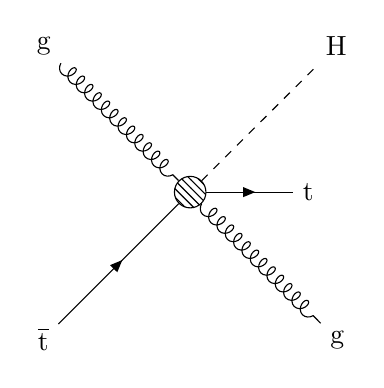
\begin{tikzpicture}
  \begin{feynman}
    \diagram [horizontal=a to b, arrow size=1pt] {
      a [particle=\(\Pg\)] -- [gluon] o [blob, minimum size = 0.4cm] -- [scalar] b [particle=\(\PH\)],
      c [particle=\(\overline \Ptop\)] -- [fermion] o        -- [gluon] d [particle=\(\Pg\)],
    };
    \vertex [right=1.5cm of o] (e) {\(\Ptop\)};
    \diagram* [arrow size=1pt] {
      (o) -- [fermion] (e);
    };
  \end{feynman}
\end{tikzpicture}
\end{document}
